% 第三章：极坐标共形解耦表示、纤维丛构图与凸支撑路由（合并数学依据与核心算法设计）
\section{Warped-Product Representation, Topology, and Routing}
\label{sec:design}

\begin{figure*}[t]
  \centering
  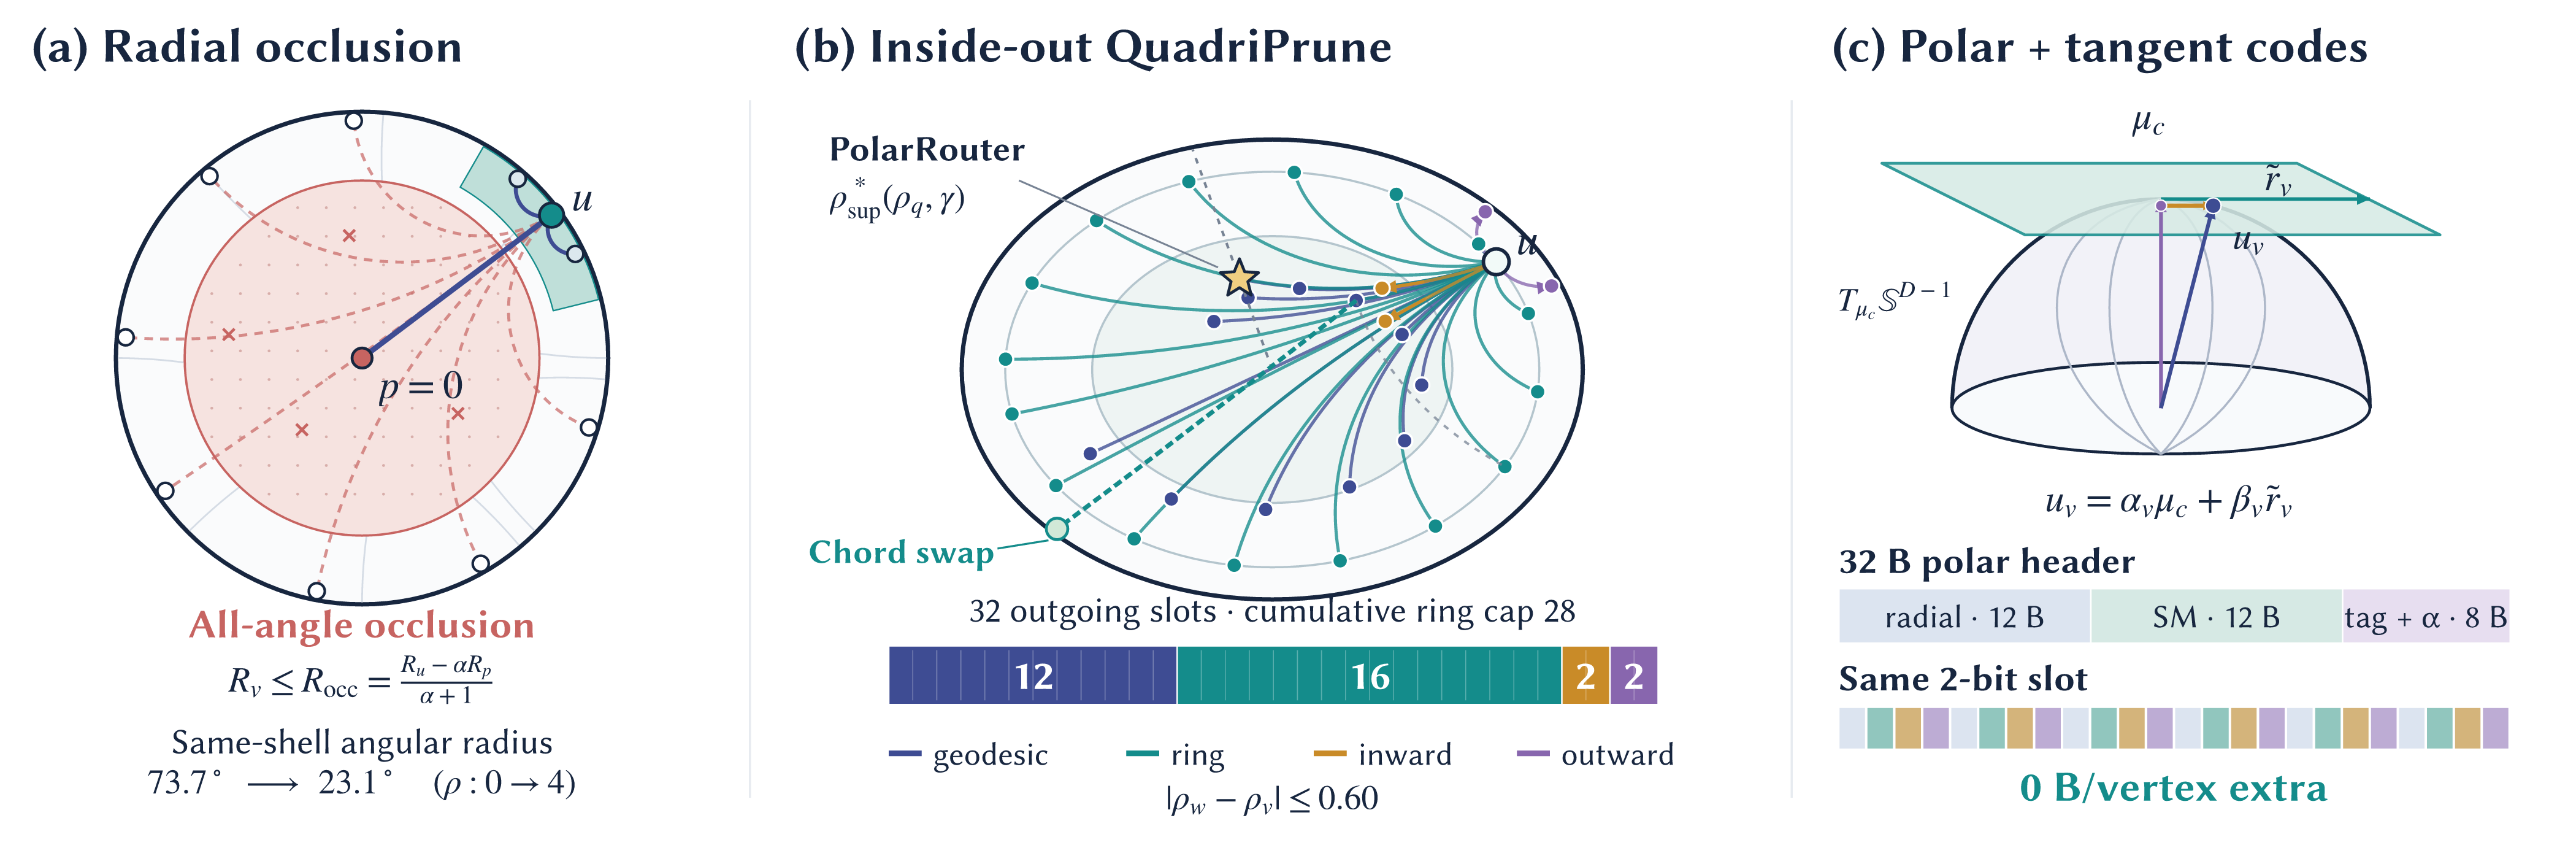
\includegraphics[width=0.95\textwidth]{pelorus_geometry.png}
  \caption{Geometric design of \rquiver{}. (a)~An origin hub exposes all-angle inner-ball occlusion and a shrinking same-shell angular cap ($\alpha=1.2$). (b)~A 32-slot example allocates 12 geodesic, 16 ring, two inward, and two outward links, with a cumulative ring cap of 28. \texttt{PolarRouter} selects ray-support entries, and chord swaps attach islands while preserving the BFS tree. (c)~Tangent encoding reuses the polar header and directional bitplanes, with cosine-error multiplier $\beta_{q,c}\beta_v$. On synthetic {Clustered-Narrow}, Recall@10 rises from $34.22\%$ to $99.385\%$ at $L=256,B=128$.}
  \label{fig:geometry_overview}
\end{figure*}

Figure~\ref{fig:geometry_overview} summarizes the geometry and representation. We co-design \rquiver{}'s representation, topology, and router by pairing each curved-manifold pathology directly with its resolving primitive (complete proofs in the supplemental material).

\subsection{Conformal Flip Analysis and 32-Byte Polar Header}
\label{subsec:polar_layout}

Let $\varepsilon_\angle(q, v) \triangleq \hat{\gamma}(u_q, u_v) - \gamma_{qv}$ be directional error in $\widehat{P}_{\mathbb{B}}(q, v) = R(r_q, r_v) + W(r_q, r_v)(1 - \hat{\gamma}(u_q, u_v))$.
For the uncalibrated bilinear product $\langle \hat{u}_q/\sigma_q, \hat{u}_v/\sigma_v\rangle$ (before calibration in~\eqref{eq:sm_calibration}) with $e_z = \hat{u}_z / \sigma_z - u_z$, bilinear decomposition~\cite{bussgang1952crosscorrelation,xiao2026decisions} gives $\varepsilon_\angle(q, v) = \eta_q(u_v) + \eta_v(u_q) + \xi_{qv}$ ($\eta_q(u_v) = \langle e_q, u_v\rangle$, $\eta_v(u_q) = \langle u_q, e_v\rangle$, $\xi_{qv} = \langle e_q, e_v\rangle$).
In flat cosine search ($W \equiv 1$), $\eta_q(u_x) - \eta_q(u_y) = \langle e_q, u_x - u_y\rangle$ has variance $(u_x - u_y)^\top\Sigma_q(u_x - u_y)$ ($\Sigma_q = \Cov(e_q)$, $\|\Sigma_q\|_2 = O(1/D)$), giving standard deviation $O(\|u_x - u_y\|_2/\sqrt{D})$~\cite{xiao2026decisions}. On $\Bball$,~\eqref{eq:cross_shell_var} models one term before calibration. A hop-score inversion also depends on the true pairwise margin.

\begin{theorem}[Conformal Flip Criterion, Depth Invariance, and Lorentz-MIPS Blowup]
\label{thm:conformal_flip}
Let $q, x, y \in \Bball$ ($r_q > 0$) satisfy $\Delta_P(q; x, y) \triangleq P_{\mathbb{B}}(q, y) - P_{\mathbb{B}}(q, x) > 0$ with real-valued radial scalars $(r_z, f_z)$ (FP32 rounding bounds in the supplemental material). Then:
(1)~\textbf{Query depth invariance:} $\widehat{P}_{\mathbb{B}}(q, y) \le \widehat{P}_{\mathbb{B}}(q, x)$ holds iff $r_y f_y \varepsilon_\angle(q, y) - r_x f_x \varepsilon_\angle(q, x) \ge \Delta_P / (2 r_q f_q)$. On an isobathic shell ($r_x = r_y = r>0$), this reduces to $\varepsilon_\angle(q, y) - \varepsilon_\angle(q, x) \ge \gamma_{qx} - \gamma_{qy}$, independent of both radii at fixed directions and estimates.
(2)~\textbf{Cross-shell non-cancellation:} For arbitrary $\Sigma_q = \Cov(e_q)$ under bilinear error, mismatched weights $d_q = W(r_q, r_y) - W(r_q, r_x)$ leave uncancelled query variance $d_q^2 u_x^\top\Sigma_q u_x$ at $u_x = u_y$. Specializing to $\Sigma_q = \frac{\kappa_q}{D}(I_D - u_q u_q^\top)$ gives
\begin{equation}
  \begin{aligned}
    &\Var_{e_q}\!\bigl(d_q\eta_q(u_x)\mid u_x=u_y\bigr)\\
    &\quad=\frac{4\kappa_q}{c^2D}\sinh^2\rho_q
      \bigl(\sinh\rho_y-\sinh\rho_x\bigr)^2(1-\gamma_{qx}^2),
  \end{aligned}
  \label{eq:cross_shell_var}
\end{equation}
growing as $\Theta(e^{2\rho_q + 2\max(\rho_x,\rho_y)}/D)$ for fixed shell gap and $1 - \gamma_{qx}^2 > 0$, shrinking to $O(\delta_\rho^2 W^2)$ within $|\rho_y - \rho_x| \le \delta_\rho$, and vanishing at $e_q = 0$.
(3)~\textbf{Spatial Lorentz-MIPS scaling:} Under $\Cov(\epsilon_v) = \Theta(\|\tilde{z}_v\|_2^2 / D)I_D$, quantizing $\tilde{z} = \frac{1}{\sqrt{c}}\sinh\rho_z\,u_z \in \R^D$ on $\Lmod$ without polar separation incurs error standard deviation $\Theta(\frac{1}{c\sqrt{D}}\sinh\rho_q\sinh\rho_v)$ even at $\theta_{qv} = 0$.
\end{theorem}
\begin{proof}[Proof Sketch]
Exact $R, W$ give $\widehat{P}_{\mathbb{B}}(q, v) - P_{\mathbb{B}}(q, v) = -2 r_q f_q r_v f_v \varepsilon_\angle(q, v)$, so dividing by $2 r_q f_q > 0$ proves~(1).
Isolating $d_q\eta_q(u_x)$ yields~\eqref{eq:cross_shell_var}, while $\|\tilde{z}_v\|_2 = c^{-1/2}\sinh\rho_v$ scales spatial steps.
\end{proof}

\paragraph{32-Byte \texttt{PolarNodeMeta} Header.}
Guided by Theorem~\ref{thm:conformal_flip}, \rquiver{} projects $\Lmod \to \Bball$ via~\eqref{eq:lorentz_isometry} and pairs 2-bit {SM} bitplanes ($2\lceil D / 64\rceil \times 8$\,B) with a 32-byte header:
(1)~unquantized FP32 radial scalars $(r_v, F_v, \rho_v)$ ($12$\,B, $F_v = (1 - c r_v^2)^{-1} = f_v/2$, computed in FP64),
(2)~FP32 {SM} scalars $(a_v, \delta_v, \sigma_v)$ ($12$\,B) for hop scoring and \textsc{Stage-0.5}, and
(3)~a 32-bit word packing 20-bit $s_v$ and 12-bit $\text{cone\_id}$ (\texttt{0x0FFF} for global {SM}) plus an FP32 slot ($8$\,B) storing $\alpha_v = \langle u_v, \mu_c\rangle$ on cones or $(D + 3 s_v)^{-1/2}$ on global legacy paths.
At $D = 768, M_0 = 32$ (Table~\ref{tab:node_layout}), logical per-vertex navigation state is $384$\,B with \texttt{SymSketch256} ($517.0$\,MB page-co-located, $2.07\times$ below {Polar-SQ8} at $1{,}069.0$\,MB and $6.52\times$ below {Polar-FP32} at $3{,}373.0$\,MB) or $352$\,B without the sketch ($485.0$\,MB split, $2.20\times$ and $6.95\times$ smaller), separating traversal from the $3{,}072.0$\,MB cold FP32 rerank store.

\begin{table}[t]
  \centering
  \caption{Per-vertex logical hot navigation payload and {Cohere-1M} byte reconciliation ($D=768, M_0=32, N=10^6$).}
  \label{tab:node_layout}
  \footnotesize
  \setlength{\tabcolsep}{3.5pt}
  \begin{tabularx}{\linewidth}{@{}>{\raggedright\arraybackslash}Xrrrr@{}}
    \toprule
    & Header/code/edges & Logical & Hot & Total \\
    Representation & B/vertex & B/vertex & MB & MB \\
    \midrule
    Polar-FP32 & 32/3,072/128 & 3,232 & 3,373 & 3,373 \\
    Polar-SQ8 & 32/768/128 & 928 & 1,069 & 4,141 \\
    \rquiver{}-Split & 32/192/128 & 352 & 485 & 3,557 \\
    \textbf{\rquiver{}} & \textbf{64/192/128} & \textbf{384} & \textbf{517} & \textbf{3,589} \\
    \bottomrule
  \end{tabularx}
  \par\smallskip
  {\scriptsize\raggedright The logical payload counts 32 active edges. Fixed-stride adjacency reserves 64 IDs/vertex ($256$\,MB), plus $4$\,MB for degrees and $0.975$\,MB for routing. Page-co-located codes and headers add $256$\,MB. Total includes one $3{,}072$\,MB FP32 vector store, reused for navigation by Polar-FP32. SQ8/FP32 hot counts include $8$\,MB of inverse norms and exclude an unused $192$\,MB 2-bit benchmark allocation. Totals are index-array accounting in decimal MB. Process RSS also includes benchmark and allocator overhead. An active cone dictionary adds $4CD$ bytes ($0$ on this dataset).\par}
\end{table}

\subsection{Boundary Margin Collapse and Purity-Gated \texttt{ResidualConeDict}}
\label{subsec:tangent_cone}

Even when $e_q = 0$, candidate quantization noise persists inside tight boundary cones around unit axis $\mu_c \in \Sunit$.
Decomposing $u_v = \alpha_v\mu_c + \beta_v\tilde{r}_v$ ($\alpha_v = \langle u_v, \mu_c\rangle$, $\beta_v = \sqrt{1 - \alpha_v^2}$, $\tilde{r}_v \in T_{\mu_c}\Sunit \cap \Sunit$) and $u_q = \alpha_{q,c}\mu_c + \beta_{q,c}\tilde{r}_{q,c}$ writes $\gamma_{qv} = \alpha_{q,c}\alpha_v + \beta_{q,c}\beta_v\langle \tilde{r}_{q,c}, \tilde{r}_v\rangle$.

\begin{theorem}[Tangent-Cone Error Propagation and Fixed-Budget Admission]
\label{thm:tangent_cone}
Consider same-shell candidates $x, y$ with weight $W = W(r_q, r) > 0$, common $\alpha = \sqrt{1 - \beta^2}$ ($\beta, \beta_{q,c} > 0$), and $\Delta_{\tilde{r}} = \langle \tilde{r}_{q,c}, \tilde{r}_y - \tilde{r}_x\rangle \ne 0$ under conditional zero-mean errors:
(1)~\textbf{Pairwise margin and covariance:} The true margin is $W\beta_{q,c}\beta|\Delta_{\tilde{r}}|$. For global cosine errors $g_x, g_y$ with $V_g = \Var(g_y) + \Var(g_x) - 2\Cov(g_y, g_x) > 0$, $\MNR_{\mathrm{global}} = \beta_{q,c}\beta|\Delta_{\tilde{r}}| / \sqrt{V_g}$, collapsing as $\sqrt{V_g}/(\beta_{q,c}\beta|\Delta_{\tilde{r}}|) \to \infty$.
(2)~\textbf{Fixed-budget admission under exchangeable ranks:} If the retained pool holds $N_c(L) \ge B$ cone members including $k_c(L)$ true neighbors and all $B$ rerank slots are drawn from them under a conditional uniform rank permutation, expected true-neighbor admission is $k_c(L) B / N_c(L)$, decreasing iff $k_c(L) / N_c(L)$ decreases.
(3)~\textbf{Exact tangent-error attenuation:} With real-valued axial scalars in
\begin{equation}
  \hat{\gamma}_{\mathrm{cone}}(q, v) \triangleq \alpha_{q,c}\alpha_v + \beta_{q,c}\beta_v\,\hat{\gamma}_{\mathrm{asym}}(\tilde{r}_{q,c}, \tilde{r}_v)
  \label{eq:cone_estimator}
\end{equation}
and $e_v = \hat{\gamma}_{\mathrm{asym}}(\tilde{r}_{q,c}, \tilde{r}_v) - \langle \tilde{r}_{q,c}, \tilde{r}_v\rangle$, cosine error equals $\beta_{q,c}\beta_v e_v$ pointwise. For $V_r = \Var(e_y) + \Var(e_x) - 2\Cov(e_y, e_x) > 0$, $\MNR_{\mathrm{cone}} = |\Delta_{\tilde{r}}| / \sqrt{V_r}$ and $\MNR_{\mathrm{cone}} / \MNR_{\mathrm{global}} = \sqrt{V_g} / (\beta_{q,c}\beta\sqrt{V_r})$. Tangent codes improve MNR exactly when $V_g>(\beta_{q,c}\beta)^2 V_r$.
\end{theorem}
\begin{proof}[Proof Sketch]
Axial terms $\alpha_{q,c}\alpha$ cancel in $\Psi_{\mathrm{rank}}$, so $\Var(X - Y) = \Var(X) + \Var(Y) - 2\Cov(X, Y)$ gives $W^2 V_g$ globally and $W^2\beta_{q,c}^2\beta^2 V_r$ under~\eqref{eq:cone_estimator}, while uniform ranks admit each cone member with probability $B / N_c(L)$.
\end{proof}

\rquiver{} adapts residual normalization~\cite{jegou2011pq} to $\Sunit$ as a fail-safe for clustered boundary cones without perturbing diffuse contrastive manifolds~\cite{wang2020understanding,betser2026infonce,xiao2026decisions} via a two-stage build check over $\min(N, 8{,}192)$ non-origin samples:
(1)~shallow distributions ($p_{90}(\rho) < 1.0$) bypass residual encoding immediately because boundary Jacobian amplification is mild;
(2)~otherwise ($p_{90}(\rho) \ge 1.0$), a spherical leader pass ($\tau_{\mathrm{lead}} = 0.91$, $\le 1{,}024$ seeds) and two spherical-mean rounds ($\langle u_s, \mu_c\rangle \ge 0.94$) retain up to $C \le 512$ axes meeting support $\operatorname{clamp}(\lfloor N_{\mathrm{samp}}/1024\rfloor, 3, 12)$ and purity $\bar{\alpha}_c \ge 0.955$, exiting with $0$ cones if no cluster passes purity.
Vertices with $\alpha_v \ge 0.94$ store the 2-bit {SM} code of $\tilde{r}_v$ in the existing bitplane slot and record $\text{cone\_id}$ in the 12-bit header (\textbf{0\,B/vertex} overhead, $\beta_v^2 \le 0.1164$).
Among the eight primary workloads, MERU-1M and WordNet-Hazy exit at the depth check. Cohere-1M, OpenAI-1536 and the two isotropic sets exit at the purity check. Both clustered sets activate 256 cones ($4CD$ bytes or $0.50$\,MiB at $D=512$).

\subsection{Hyperbolic Vamana Pathologies, QuadriPrune, and Chord-Swap Repair}
\label{subsec:compass}

For {Vamana} pruning~\cite{subramanya2019diskann}, triangle inequalities give a sufficient inner-ball bound. The same-shell formula assumes an origin neighbor. On Cohere, $R_{\mathrm{occ}}\le1.01$, below the first-percentile depth of $1.45$. The bound leaves occlusion farther out unresolved.

\begin{theorem}[Radial Occlusion, Cone Contraction, Escape Cap, and Surrogate Bias]
\label{thm:vamana_pathologies}
On $\Bball$ ($-c < 0$) under pruning slack $\alpha > 1$:
(1)~\textbf{Radial occlusion and cone contraction:} If outer vertex $u$ ($R_u > 0$) admits interior neighbor $p$ ($R_p < R_u / \alpha$), then every $v$ inside $R_v \le R_{\mathrm{occ}} \triangleq (R_u - \alpha R_p)/(\alpha + 1)$ satisfies $\alpha\,d_{\mathbb{B}}(p, v) \le d_{\mathbb{B}}(u, v)$ across all $\theta_{pv} \in [0, \pi]$.
Specifically under negative curvature, for $R_u = R_v = R$ ($\rho = \sqrt{c}R$) and $p = 0$ ($\alpha \in (1, 2)$), $\alpha\,d_{\mathbb{B}}(0, v) \le d_{\mathbb{B}}(u, v)$ holds whenever
\begin{equation}
  \sin(\theta_{uv}/2) \ge \sinh(\tfrac{\alpha}{2}\rho)/\sinh(\rho) \sim e^{-(2-\alpha)\rho/2},
  \label{eq:cone_contraction}
\end{equation}
shrinking the unoccluded cone from $73.7^\circ$ ($c \to 0^+$) to $23.1^\circ$ ($\rho = 4$) and $10.4^\circ$ ($\rho = 6$) at $\alpha = 1.2$.
(2)~\textbf{Angular escape condition:} Candidate $v$ satisfies $d_{\mathbb{B}}(q, v) < R_q$ iff $\gamma_{qv} > \gamma_{\mathrm{esc}}(R_q, R_v) \triangleq \tanh(\sqrt{c}R_v / 2)/\tanh(\sqrt{c}R_q)$. Equality gives $d_{\mathbb{B}}(q,v)=R_q$ for positive depths.
(3)~\textbf{Surrogate bias:} Affine surrogates $\hat{d} = a d + b$ ($a > 0$) yield margin $a[d(u, v) - \alpha d(w, v)] + (1 - \alpha)b$ ($b > 0$ under-prunes, $b < 0$ over-prunes). The geodesic test $\alpha d(w,v)\le d(u,v)$ is equivalent to $P_\alpha(P_{\mathbb B}(w,v))\le P_{\mathbb B}(u,v)$, where $P_\alpha(x)=\frac{2}{c}[\cosh(\alpha\arccosh(1+cx/2))-1]$. Since $P_\alpha(x)>\alpha x$ for $x>0$, using $\alpha P_{\mathbb B}(w,v)$ on the left over-prunes.
\end{theorem}
\begin{proof}[Proof Sketch]
Triangle-inequality sufficient bounds $d_{\mathbb{B}}(p, v) \le R_p + R_v$ and $d_{\mathbb{B}}(u, v) \ge R_u - R_v$ give $R_{\mathrm{occ}}$, while $\sinh(\frac{\sqrt{c}}{2}d_{\mathbb{B}}(u, v)) = \sinh\rho\sin(\theta_{uv}/2)$ yields~\eqref{eq:cone_contraction}.
Expanding $\cosh(\sqrt{c}d_{\mathbb{B}}(q, v)) < \cosh\rho_q$ gives $\gamma_{\mathrm{esc}}$, and $\hat{d}(u, v) - \alpha\hat{d}(w, v)$ isolates $(1 - \alpha)b$.
\end{proof}

\begin{algorithm}[t]
\caption{Warped-Product Construction \& Chord-Swap Repair}
\label{alg:compass_build}
\footnotesize
\begin{algorithmic}[1]
\Require Dataset $\mathcal{X} \subset \Bball$, max out-degree $M_0 = 2M$, build beam $L_c$, slack $\alpha > 1$
\Ensure Graph $G = (V, E)$ with maximum degree $M_0$ and measured entry-reachable set $\mathcal{R}$
\State Build \texttt{PolarNodeMeta}, purity-gated \texttt{ResidualConeDict}, 2-bit {SM}, and \texttt{PolarRouter}
\State Sort $\pi = (v_1, \dots, v_N)$ by $\rho_{v_1} \le \dots \le \rho_{v_N}$ with empty adjacency lists
\For{consecutive radial wave $B_t \subset \pi$ ($\le 256$ vertices) ordered inside-out}
  \For{each $u \in B_t$ in parallel}
    \State $\mathcal{C}_u \gets \textsc{PolarBeamSearch}(G, u, L_c)$ using 2-bit proxy $\widehat{P}_{\mathbb{B}}$
    \State Partition $\le M_0$ edges via \textbf{QuadriPrune}: geodesic fiber (cap $\max(1, \lfloor \frac{3}{8}M_0\rfloor)$) via~\eqref{eq:dom_geo}, shielded ring (cumulative cap $\lfloor \frac{7}{8}M_0\rfloor$, $|\rho_w - \rho_v| \le 0.60$), and inward/outward elevators via~\eqref{eq:elevator_obj} plus fallback fill
    \State Add reverse edges $v \to u$ for $v \in N^+(u)$, re-pruning if $\deg^+(v) > M_0$
  \EndFor
\EndFor
\State Final-prune lists to $M_0$, then $(\mathcal{R}, \texttt{parent}) \gets \textsc{DirectedBFSTree}(G, \text{entry\_hub})$
\For{each $u \in \pi$ with $u \notin \mathcal{R}$}
  \State Find reachable $p \in \mathcal{R}$ in $N^+(u)$, hubs, or 256-vertex core prefix with free slot or removable chord (if none exists, \textbf{continue})
  \State Append $p \to u$ if $\deg^+(p) < M_0$, else swap chord $p \to w^\star$ ($\texttt{parent}[w^\star] \ne p \land \deg^-(w^\star) \ge 2$) with $p \to u$
  \State $\texttt{parent}[u] \gets p$, then expand $(\mathcal{R}, \texttt{parent})$ via incremental {BFS} from $u$
\EndFor
\State \Return fixed-stride graph $G$, reachable set $\mathcal{R}$, and $4096$\,B \texttt{HotSmPage} store
\end{algorithmic}
\end{algorithm}

\paragraph{Inside-Out Seeding, QuadriPrune, and Chord-Swap Repair.}
Algorithm~\ref{alg:compass_build} builds full-database router seeds before connecting $\le 256$-vertex inside-out waves across four cumulative channels ($M_0=32$). The channel weights and shell cutoffs are empirical constants held fixed across datasets.
(1)~\emph{Geodesic fiber} ($12$ slots): with $\tilde{d} = \sqrt{c}d_{\mathbb{B}}$, $\ell_\angle(x, y) = 1 - \hat{\gamma}(u_x, u_y)$, $\Delta_{\mathrm{stem}}(u, v, w) = \max(0, |\rho_u - \rho_v| - |\rho_w - \rho_v|)$, and $\tilde{d}_{\mathrm{eff}}(u, v, w) = \max(0, \tilde{d}(u, v) - \Delta_{\mathrm{stem}})$, neighbor $w$ dominates $v$ iff
\begin{equation}
  \bigl[\ell_\angle(w, v) \le \ell_\angle(u, v)\bigr] \;\land\; \bigl[\alpha\,\tilde{d}(w, v) \le \tilde{d}_{\mathrm{eff}}(u, v, w)\bigr],
  \label{eq:dom_geo}
\end{equation}
enforcing the angular guard and rejecting $\alpha|\rho_w - \rho_v| > \tilde{d}_{\mathrm{eff}}$ in $O(1)$ arithmetic.
(2)~\emph{Shielded ring} ($28$ cumulative slots): orders candidates by $\ell_\angle(u, v) + 0.85|\rho_u - \rho_v|$ and limits $\alpha\ell_\angle(w, v) \le \ell_\angle(u, v)$ to $|\rho_w - \rho_v| \le 0.60$. Only neighbors within this depth gap can suppress a ring candidate.
(3)--(4)~\emph{Inward/outward elevators} (splitting remaining $h = M_0 - s$ slots as $\lfloor h/2\rfloor$ inward on $\rho_v < \rho_u - 0.18$ and outward on $\rho_v > \rho_u + 0.18$, with dominators $\rho_w < \rho_u - 0.10$ / $\rho_w > \rho_u + 0.10$): minimize
\begin{equation}
  J_{\mathrm{elev}}(u, v) \triangleq \ell_\angle(u, v) + 0.15\bigl||\rho_v - \rho_u| - 0.65\bigr|,
  \label{eq:elevator_obj}
\end{equation}
followed by diversity fill ($\ell_\angle + 0.25|\rho_u - \rho_v|$, $|\rho_w - \rho_v| \le 1.0$) and ordered fill (with fixed dataset-independent quotas and tolerances; at constant depth, elevator sets are empty and the ring prunes by angle).
The chord-swap pass repairs the $521\text{--}628$ zero-in-degree boundary islands on {Cohere-1M} while preserving tree edges, achieving $1{,}000{,}000 / 1{,}000{,}000$ directed {BFS} reachability from the entry hub ($0$ islands) across all 21 million-scale {Zen~4} graphs in $<0.3$\,s.

\subsection{Ray Strong Convexity and \texttt{PolarRouter}}
\label{subsec:router}

\begin{proposition}[Radial Lower Bound and Constrained Radial Minimizer]
\label{prop:geodesic_apex}
For $q \in \Bball$ at depth $\rho_q$:
(1)~$P_{\mathbb{B}}(q, v) \ge P_{\mathrm{rad}}(r_q, r_v) \triangleq (r_q - r_v)^2 f_q f_v = \frac{2}{c}(\cosh|\rho_q - \rho_v| - 1)$ for all $v \in \Bball$.
(2)~Along a ray $\{v(\rho) : \rho \in \R\}$ of alignment $\gamma = \langle u_q, \mu_a\rangle$, $g_\gamma(\rho) \triangleq \cosh\rho_q\cosh\rho - \gamma\sinh\rho_q\sinh\rho$ satisfies $g_\gamma''(\rho) = g_\gamma(\rho) \ge \cosh(\rho_q - |\rho|) \ge 1$ ($1$-strong convexity on $\R$) and attains its unique minimizer on $[\rho_{\min}, \rho_{\max}] \subset [0, \infty)$ at $\rho_{\mathrm{sup}}^* = \operatorname{clip}_{[\rho_{\min},\rho_{\max}]}(\rho^*)$ where
\begin{equation}
  \rho^*(\rho_q, \gamma) = \atanh\bigl(\tanh\rho_q \cdot \max(\gamma, 0)\bigr),
  \label{eq:geodesic_apex}
\end{equation}
specializing hyperbolic right-triangle projection to bounded radial support.
\end{proposition}
\begin{proof}[Proof Sketch]
$\gamma_{qv} \le 1$ gives~(1). Differentiating twice gives $g_\gamma''(\rho) \ge \cosh(\rho_q - |\rho|) \ge 1$, $g_\gamma'(\rho) = 0$ yields~\eqref{eq:geodesic_apex}, and clamping follows by strict convexity.
\end{proof}

Avoiding origin-medoid traps (Theorem~\ref{thm:vamana_pathologies}(2)), \texttt{PolarRouter} builds $C = \min(N, \operatorname{clamp}(\lfloor N/100\rfloor, 64, 2048))$ Tammes-style {SM} landmarks~\cite{tammes1930origin} ($64$ coarse landmarks with $128$-cone shortlists when $C > 256$, plus $16$ origin hubs) crossed with $8$ quantile shells ($16{,}384$ cells $\times 8$ IDs at $N = 10^6$), seeding shell representatives via $\rho_{\mathrm{sup}}^*(\rho_q, \gamma)$ over sampled positive database depths and scanning fine cones directly when a dimension-scaled isotropy guard detects low coarse alignment (\S\ref{subsec:eval_ablation}). Validation queries can select hubs alone or full routing jointly with $(L,B)$ for each target and thread count.
